
%% This is a skeleton file demonstrating the use of IEEEtran.cls
%% (requires IEEEtran.cls version 1.7 or later) with an IEEE journal paper.
%%
%% Support sites:
%% http://www.michaelshell.org/tex/ieeetran/
%% http://www.ctan.org/tex-archive/macros/latex/contrib/IEEEtran/
%% and
%% http://www.ieee.org/


\documentclass[conference]{IEEEtran}
\usepackage{blindtext}
\usepackage{graphicx}
\graphicspath{ {images/} }
\usepackage{float}
\usepackage{url}
\usepackage{cite}


\begin{document}
%
% paper title
% can use linebreaks \\ within to get better formatting as desired
\title{Is Filecoin a \$257 million Ponzi scheme?}
%
%
% author names and IEEE memberships
% note positions of commas and nonbreaking spaces ( ~ ) LaTeX will not break
% a structure at a ~ so this keeps an author's name from being broken across
% two lines.
% use \thanks{} to gain access to the first footnote area
% a separate \thanks must be used for each paragraph as LaTeX2e's \thanks
% was not built to handle multiple paragraphs
%

\author{
\IEEEauthorblockN{Marc Juchli}
\IEEEauthorblockA{Faculty of Electrical Engineering,\\ Mathematics and Computer Science\\
Delft University of Technology\\
m.b.juchli@student.tudelft.nl}
\and
\IEEEauthorblockN{Johan A. Pouwelse}
\IEEEauthorblockA{Parallel and Distributed Systems Group \\ Department of Software and Computer Technology \\
Delft University of Technology\\
j.a.pouwelse@tudelft.nl}
}


% The paper headers
%\markboth{The Culture Clash, September~2016}%
%{}
% The only time the second header will appear is for the odd numbered pages

% make the title area
\maketitle

\begin{abstract}
%\boldmath

Centralized storage providers are dominating the storage market and host a major part of internet data.
In the recent blockchain era, the idea of decentralized storage was connected with the incentive that leads to a decentralized storage market.
This paper analyzes Filecoin's ICO and its technical capabilities, as described in detail in its Whitepaper.
Moreover, the InterPlanetary File System (IPFS) project will be considered in detail; this is a peer-to-peer hypermedia protocol which Filecoin uses as its the underlying data store.
Further, the question of whether or not Filecoin is an economically feasible project is discussed by means of extending the work of a hypothetical risk analysis, considering the possibility of a Ponzi scheme and finally, sketching a back-of-the-envelope calculation.
The paper uncovers unattractiveness during the ICO which leaves investors without any control after their investment.
Filecoin's Whitepaper introduces novel concepts and predecessor projects from the team members proof technical capabilities.
We highlight that the integration of IPFS into Filecoin can be achieved by exploiting the capabilities provided by Bitswap.
The feasibility in economical terms is hard to predict and the biggest hurdles is probably going to be the acceptance from the users.
In addition, Filecoin shows certain characteristics of a Ponzi scheme but the trust built by the team members in the past leads to believe otherwise.

\end{abstract}

\begin{IEEEkeywords}
filecoin, crypto-currency, ipfs, libp2p, decentralized storage, ico, proof-of-spacetime, ponzi scheme.
\end{IEEEkeywords}

\IEEEpeerreviewmaketitle

\section{Introduction}

\begin{quote}"A MASSIVE AMOUNT OF STORAGE SITS UNUSED IN DATA CENTERS AND HARD DRIVES AROUND THE WORLD." \cite{filecoin-io}\end{quote}
With this slogan, Protocol Labs is about to disrupt the storage market by using \textit{proof-of-spacetime} as their driving source.
The Filecoin project describes a decentralized storage market in which anyone, worldwide, is able to participate as a storage provider.
This concept is so promising that it has convinced investors to provide a total of \$257 million –-- so far the biggest initial coin offering (ICO) as of today (September 2017).
However, the concept of a decentralized storage market is not novel.
Others\cite{tribler}\cite{mojo-nation} have tried in the past, yet were not able to reach Filecoin's advertised scaling capability, and eventually failed.
More recent projects\cite{storj}\cite{sia} are currently working towards building a similar system with conceptual differences which are explained briefly in this paper.

This paper aims to analyze the Filecoin project primarily with regard to its technical aspects, and secondarily, its economic aspects.
The most relevant financial figures relating to the Filecoin ICO are highlighted and then followed by suggested reasons for the exceptionally large investment sums by reference to heavily discussed topics in social media channels.
A number of sections from the Simple Agreement for Future Tokens (SAFT) are then discussed; they include terms which might be unattractive to the unaware investor and benefit the founder team of Filecoin.
Regarding Filecoin's technical potential, we mainly focus on what is proposed in the Whitepaper\cite{filecoin}.
Thereby, we aim to uncover potential weaknesses but also highlight strengths.
In addition, the novel \textit{proof-of-spacetime} consensus algorithm is highlighted and compared with consensus proposals from projects such as StorJ and Sia.
Moreover, we explore  the details of the InterPlanetary File System (IPFS) project, a peer-to-peer hypermedia protocol which is used as the underlying data store of Filecoin.
Not only do we set out the technical foundation, but we also explain a possible way for Filecoin to use IPFS as its storage adapter by means of Bitswap\cite{bitswap}.
The feasibility in terms of economic design is briefly discussed by reference to a hypothetical risk analysis, a consideration of whether or not the ICO launch might be a Ponzi scheme, as well as with a back-of-the-envelope calculation.

The structure of this paper is as follows: Section \ref{sec:documented-failure} lays out a history of decentralized storage projects with a similar ambitions to Filecoin, but that have failed over time. 
Section \ref{sec:recent-competitors} mentions recent competitor projects that make use of a blockchain.
Subsequently, Section \ref{sec:ico-analysis} introduces the Filecoin project by analyzing the ICO including reasons for the sale and allocation of tokens.
Section \ref{sec:tech-feasibility} considers whether the promises of the Filecoin project are technically feasible or not.
Accordingly, we are then able to analyze the InterPlanetary File System (IPFS)\cite{ipfs-whitepaper} in Section \ref{sec:ipfs} and highlight possible ways means of adoption.
In Section \ref{sec:eco-feasibility}, we question the economic feasibility in a rudimentary manner and lastly draw a number of conclusions about the entire Filecoin project in Section \ref{sec:conclusion}.


\section{15 years of documented failure}
\label{sec:documented-failure}

In July 2000, long before the blockchain era, the Mojo Nation software \cite{mojo-nation} was released, with the aim of providing an \textit{emergent file store} to its users.
The project successfully deployed a decentralized storage network in an environment consisting of unmanaged nodes.
It used consistent hashing \cite{consistent-hashing} to locate nodes and data blocks.
However, the project was shut down in February 2002 due to a number of problems:
\begin{itemize}
\item \textbf{Data Availability:} the main issue was the inconsistency of data available to its users as it depended upon which server nodes were connected at any given time.
According to Maymounkov et al.\cite{peer-to-peer-xor} this could have been avoided by heuristically favoring long-lived nodes and by discriminating against newly joined nodes which show frequent \textit{join-and-leave} behavior.
\item \textbf{Firewalls and NAT}: networking hurdles such as firewalls and network address translation (NAT) prevented a substantial amount of nodes from acting as servers.
\item \textbf{Mutual distrust:} in order to enable a network of nodes to behave as designed, a \textit{motivation to cooperate} needed to be established within the network, combined with a sophisticated \textit{attack resistance} mechanism which would have prevented nodes from using the resources of other nodes without offering an equal level of service in return.
\end{itemize}
\hfill
\\
In addition, academia has been struggling to build self-organizing systems.
Tribler\cite{tribler} is based on a robust reputation and the sharing of expertise thereby, facilitating an environment where a decentralized marketplace can be thought of as something which treats storage as an asset.
In its 12-years development history, there have been many challenges. 
For example, security issues including collusion attacks\cite{tribler-hurdles} have slowed down the progress of development enormously, in particular, preventing the project from scaling up.

\section{Recent Competitors}
\label{sec:recent-competitors}
At the time of writing, a sudden glut of ICOs has appeared, some of which are projects that are destined to have the same fate as Filecoin.
Figure \ref{fig:ico-vs-venture} shows that the funds invested in ICOs have exceeded the investments made in the venture capital sector.
\begin{figure}[h]
\centering
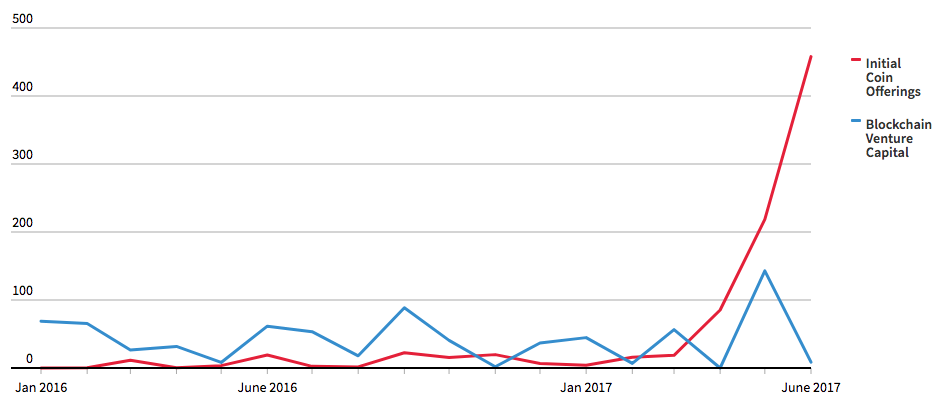
\includegraphics[width=0.45\textwidth]{ico-vs-venture}
\caption{ICOs vs Venture Capital \cite{ico-vs-venture}}
\label{fig:ico-vs-venture}
\end{figure}
The following are examples of some of the most capitalized projects to have resulted in decentralized, incentivized, and byzantine fault-tolerant storage networks which will eventually compete with centralized alternatives such as Amazon S3\cite{amazon-s3} are: StorJ\cite{storj}, Sia\cite{sia} and MaidSafe\cite{maidsafe}.
\begin{itemize}
\item \textbf{Sia}: supports on-blockchain smart contracts which define payments for hosts while providing storage. 
Payment is guaranteed once the contract has been created and ensures that the host is still paid even if the uploader never accesses the file. 
Additionally, the contract enforces penalties for hosts which go offline or lose data.
\item \textbf{Storj}: is similar to Sia but does not feature on-blockchain storage contracts; instead, it offers a pay-as-you-go model for nodes which provide storage. 
Once the host disappears or goes offline, payments are halted.
\item \textbf{MaidSAFE} goes beyond decentralized storage with a less sophisticated focus on efficiency compared to its rivals.
MaidSAFE uses a novel scheme for achieving consensus by not relying on a blockchain but instead on close group consensus and hence is not proof-of-work related.

\end{itemize}

\section{ICO analysis}
\label{sec:ico-analysis}

The Filecoin ICO started on August 10, 2017 and completed its offering on September 7, 2017.
It was the first ICO ever to comply with SEC securities regulations and hence only accredited investors were allowed to contribute (Reg. D, 506(c), see \cite{regulation-506}).
Further, the ICO was conducted using CoinList\cite{coinlist}, a platform for token sales, also built by Protocol Labs.
CoinList partners with AngelList\cite{angellist} who are responsible for legal compliance.
In total, approximately \$257'000'000 was raised, composed of \$52'000'000 from presale and \$205'800'000 from Reg D investments.
In respect of the latter category, \$135 million was raised within the first hour.

\subsection{Simple Agreement for Future Tokens}
\label{subsec:saft}
The issue of the tokens during the ICO was regulated by a Simple Agreement for Future Tokens ("SAFT"). 
This instrument provides a framework for Coinlist to grant to investors the right to redeem Filecoin tokens (FIL) in the future.
The definition of SAFT, however, also includes the following statement:
\begin{quotation}
"...a significant portion of the amount raised under the SAFTs will be used to fund the Company’s development of a decentralized storage network that enables entities to earn Filecoin (the “Filecoin Network”)" (sic).\cite{saft-agreement}
\end{quotation}
Therefore, the extent to which the development process is being funded is not explicitly mentioned, and thus is left to be decided solely by Protocol Labs Inc.
Additionally, the SAFT gives to the token intermediary, CoinList, a wide discretion as the agreement not only enables the verification of investors as accredited but also define certain \textit{events} to be transparently defined.
Transparency is certainly appreciated when funds are being transferred, but needless to say, the terms have to be fully understood by both parties.
One event, the impact of which might be underestimated by the investor, is the \textit{Dissolution Event} and is defined as follows:
\begin{quotation}
"Dissolution Event means (i) a voluntary termination of operations of the Company, (ii)
a general assignment for the benefit of the Company’s creditors or (iii) any other liquidation,
dissolution or winding up of the Company, whether voluntary or involuntary."\cite{saft-agreement}
\end{quotation}
Knowing that, at any given time, it is possible for Protocol Labs to terminate their business, the entire commercial objective of the ICO becomes fragile, as is clear from this extract from the \textit{execution plan}:
\begin{quotation}
"If immediately prior to the consummation of the Dissolution Event, the assets of the Company that remain legally available for distribution to the Purchaser and all holders of all other SAFTs (the “Dissolving Purchasers”), as determined in good faith by the Company’s board of directors, are insufficient to permit the payment to the Dissolving Purchasers of their respective Returned Purchase Amounts, then the remaining assets of the Company legally available for distribution will be distributed with equal priority and pro rata among the Dissolving Purchasers..."\cite{saft-agreement}\end{quotation}
In other words, only the \textit{remaining} assets which are legally available will be distributed in the event of a \textit{Dissolution Event}, including voluntary termination as seen in definition (i).
Unfortunately, if one considers the worst-case scenario in which Protocol Labs decide to terminate the operation after having spent all the funds available, the investors would likely be excluded from the distribution of any assets.
Similarly, if the project does not announce a \textit{Network Launch}\cite{saft-agreement} event by July 18, 2022 (including a 60-day extension), then according to definitions (i) or (iii), investors would have to expect a \textit{Dissolution Event} to be announced as a subsequent step.

\subsection{Token allocation}
\label{subsec:token-allocation}
As presented in \cite{token-sale}, Filecoin tokens are distributed to four groups of participants:
\begin{itemize}
\item 70\% to Filecoin Miners as mining block rewards once the \textit{Network Launch} has taken place
\item 15\% to Protocol Labs as its genesis allocation with 6-year linear vesting
\item 10\% to investors as its genesis allocation with linear vesting of 6 months to 3 years
\item 5\% to the Filecoin Foundation as its genesis allocation with 6-year linear vesting
\end{itemize}
The total of US\$257 million raised during the advisor presale and investor sale (see \ref{subsec:token-sale}) therefore only accounts for a maximum of 10\% of the total coins expected to be in circulation several years after the \textit{Network Launch}.
The half-life of Filecoin block rewards is set to 6 years and this will likely not change significantly for several years given that the \textit{Network Launch} requires a solid implementation of the Filcoin ecosystem.

\subsection{Token sale}
\label{subsec:token-sale}
There was a two-phase process for the distribution of SAFTs: the first phase enabled Protocol Labs as well as Filecoin's advisors to purchase SAFTs prior to the broader group of later investors. 
The latter were able to purchase in the second phase.
In the first phase, the price was fixed at 0.75 USD/FIL.
For the second phase, a pricing function was introduced:
\[ price = max(\$1, \frac{amountRaised}{\$40'000'000}) \]
The price determined by this function increased linearly according to the amount being raised, as indicated in Figure \ref{fig:sale-price}.
\begin{figure}[h]
\centering
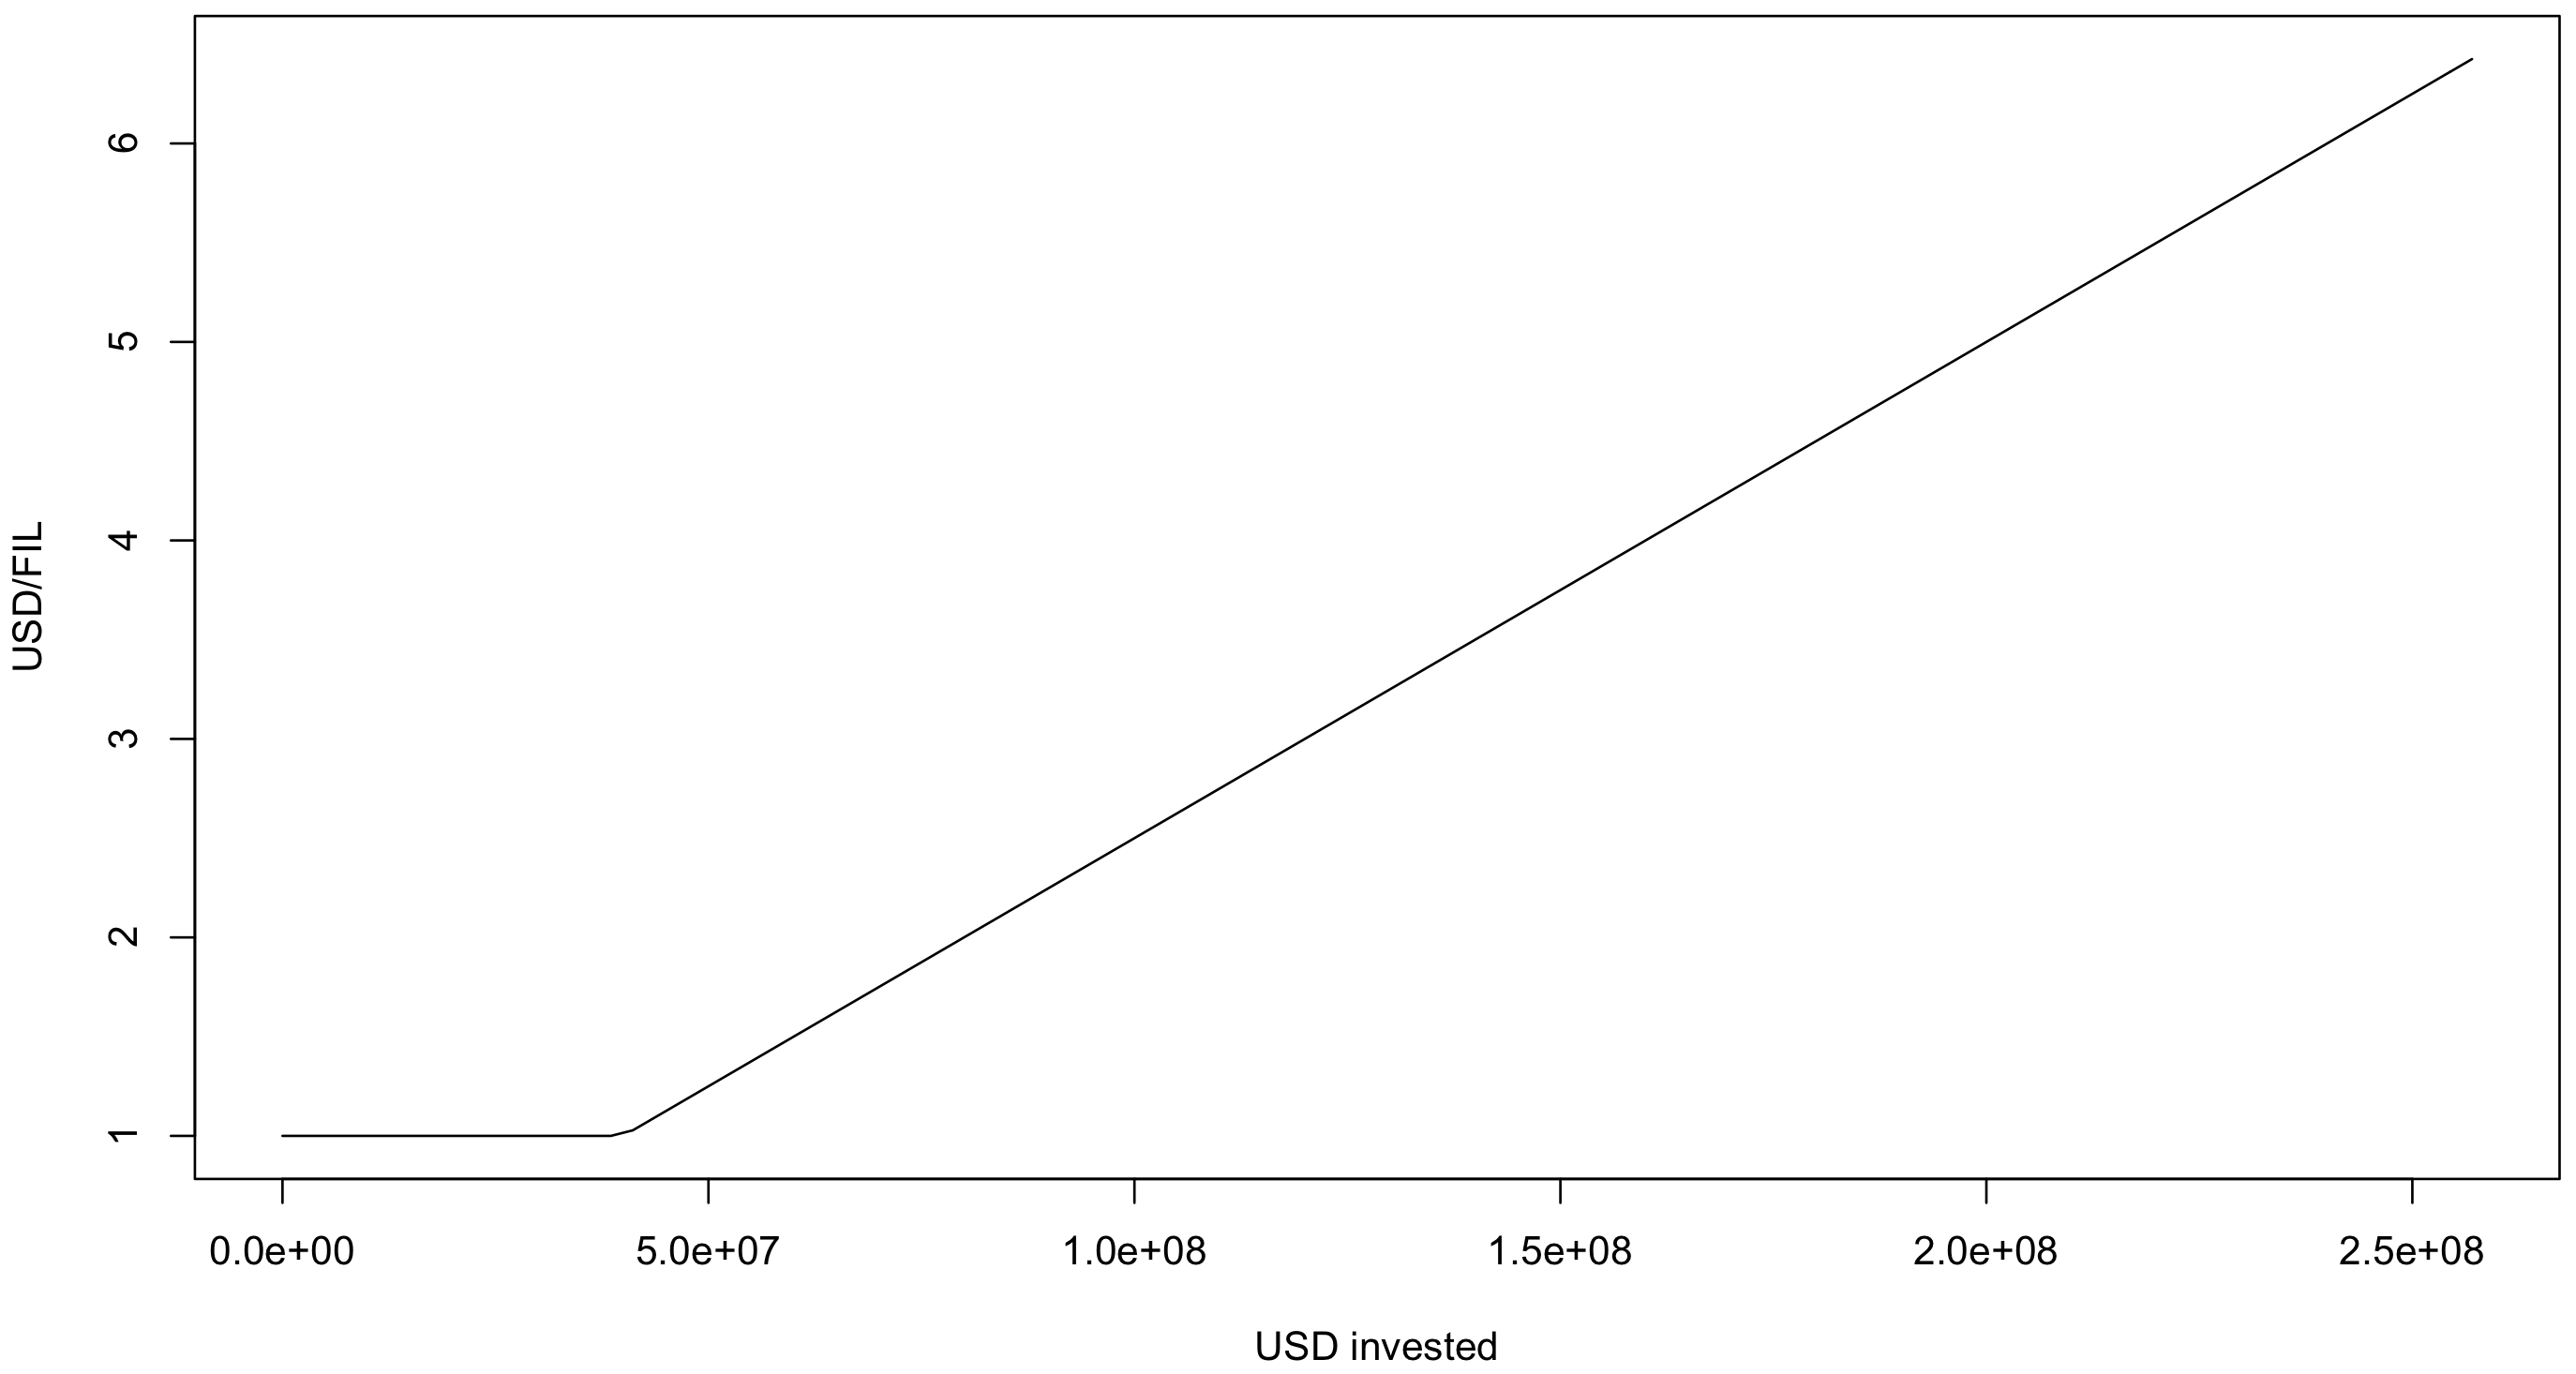
\includegraphics[width=0.45\textwidth]{filecoin-tokensale.png}
\caption{Filecoin sale price function}
\label{fig:sale-price}
\end{figure}
As a result, the closing price for investments beyond the value of \$257'000'000 can be estimated at approximately \$6.425.
Hence, advisors and Protocol Labs Inc. itself were able to purchase at a price 8.57 times lower than paid by the later investors.

\section{Is the design technically feasible?}
\label{sec:tech-feasibility}
In this section, certain technical details will be discussed and the issue of whether the decisions stated in the Whitepaper\cite{filecoin} will lead to a satisfactory outcome or whether any weaknesses in these decisions will emerge and threaten the success of the project.
Further, we aim to make comparisons with more recent decentralized storage projects involving blockchains, such as StorJ \cite{storj} and Sia \cite{sia}.

\subsection{Decentralized Storage Network}
\label{subsec:dsn}
Conceptually, a \textit{Decentralized Storage Network} (DSN) is a scheme with associated protocols that enables the aggregation and provision of data to be decentralized in a coordinated manner.
The protocols verify that the parties involved execute their operations securely and so facilitate coordination without the aid of a trusted party.
The Filecoin DSN introduces three types of participants: (1) \textit{Clients} who pay FIL tokens to the store and retrieve data, (2) \textit{Storage Miners} who pledge FIL tokens as collateral while providing amounts of storage which correspond to their value in FIL, thereby making them eligible to mine new tokens, and (3) \textit{Retrieval Miners} who provide data in response to client requests, and oftentimes also act as Storage Miners.
Further, Filecoin personifies all the participating parties which run a \textit{full nodes} as \textit{The Network ($N$)}.
Hence, the protocol scheme is being constellated as a tuple in a very suitable and abstract definition: \texttt{(Put, Get, Manage)}.
The process of storing and retrieving data is undertaken by clients using the Put or  Get Protocol.
The Network is coordinated using the Manage protocol, which serves to control the available storage, audits offered services by Storage Providers and repair possible faults.
Little is known about \texttt{Manage.AssignOrders} or \texttt{Manage.RepairOrders}, such as whether the Manage protocol follows incentive and rewards nodes in order to actively maintain the network.
However, on the basis of our research so far, we consider that the Filecoin DSN, is conceptually excellent, compared to its competitors identified in Section \ref{sec:recent-competitors}.
The simplicity of \texttt{(Put, Get, Manage)} implicitly covers additional client operations such as \texttt{PING} and \texttt{FIND\_NODE}, as defined in StorJ \cite{storj}.

The process of storing data, initiated by a client, involves splitting the data into \texttt{pieces} in order to store it within \texttt{sectors}, as part of the disk space provided by storage miners.
Conceptually, the data handling is very similar to StorJ\cite{storj} where data, after it undergoes AES256-CTR encryption executed by the client, is split into \textit{shards}.
While StorJ dynamically adjusts the size of the shards depending on the file to be stored, it is not yet known how Filecoin will approach the splitting into pieces.
Filecoin, like StorJ, delegates the encryption task to the client.
However, whereas StorJ enforces encryption in its reference client implementation, Filecoin currently has no plan for offering built-in encryption and leaves this responsibility solely to the client before they access the Filecoin network.
In order to introduce redundancy for the data to be stored, Filecoin neatly introduces a \textit{replication factor} to be chosen during the \texttt{Put} protocol, and which can be used to increase the tolerance of storage faults.
In contrast, StorJ therefore uses a distinctive \textit{mirror} method.

The guarantees and requirements laid out by the Filecoin DSN can be summarized as follows:
\begin{itemize}
\item \textit{Integrity:} In order to ensure that clients do not accept altered or falsified data, cryptographic hashes are used as a naming convention and serve as identifiers for data retrieval (\texttt{Get} protocol) and verification of content.
Unlike its competitor StorJ\cite{storj}, Filecoin does not rely on any metadata but relies on hashes only.
\item \textit{Retrievability:} after the data is successfully stored, clients are assured that the very same data can eventually be retrieved.
The $(f, m)-tolerant$ system specifies that, assuming $m$ storage miners, a maximum of $f$ faults are tolerated.
Increasing the replication factor hence implicitly increases the chances of recovery.
\item \textit{Public Verifiability and Auditability:} as storage miners are obligated to submit proofs of storage (see \ref{subsec:pos}) to the blockchain, any user can verify their validity without having access to the data.
Since \textit{proof-of-spacetime:} implicitly guarantees the continuous existence of the data on the storage miner side, no challenge-response communication is required.
Compared to StorJ\cite{storj}, the communication overhead is therefore reduced while providing the same guarantees.
\item \textit{Incentive compatibility:} like any of the projects mentioned in \ref{sec:recent-competitors}, Filecoin enforces incentive by rewarding parties which store data and punishing those who lose data.
\item \textit{Confidentiality:} as mentioned earlier in this section, Filecoin is weaker in terms of confidentiality as it fully delegates the encryption task to the client.
\end{itemize}

% Partitioning vs erasure codes \cite{sia}

\subsection{Ledger}
\label{subsec:ledger}
The \texttt{Ledger $L$} described in the Filecoin Whitepaper is represented by a native blockchain, as announced in \cite{filecoin-investor-faq}, and supports various types of data structures.
The state of the DSN is stored within an \texttt{AllocTable}, which keeps track of \texttt{pieces} and their assigned \texttt{sectors}.
The \texttt{Orderbook} is responsible for storing \texttt{Orders}, which either state a request to store data (\texttt{Bid order}), offer a service (\texttt{Ask order}) or confirm a match of bid- and ask orders in the form of a \texttt{Deal order}.
Lastly, a \texttt{Pledge} engraved in the ledger represents the collateral of the storage miner deposited in order to accept orders from the clients, as described in \ref{subsec:dsn}.
In contrast, Sia only stores storage contracts which define the terms of the agreement between the parties and therefore it relies on a variant of the Bitcoin protocol\cite{bitcoin}.
As Filecoin is clearly more diverse in terms of data structures, additional complexity in the client implementation is to be expected.
From another perspective, this decision might enable the protocol to be extended more easily as the ledger is already laid out in such a way as to handle various types of data structures.
In addition, the decision to have a native blockchain was pre-condition for the use of Proof-of-Spacetime, see \ref{subsec:pos}.
It was announced at DEVCON2 \cite{devcon2} that the Ethereum Network\cite{ethereum} would be relied upon, however this decision was later abandoned. 
This meant that there was no ERC20 token, \cite{erc20} which in turn prevents direct compatibility with Ethereum and therefore requires a bridge of some sort.

%\subsection{Fault tolerance}

\subsection{Proof-of-Spacetime}
\label{subsec:pos}
The Whitepaper\cite{filecoin} describes a novel consensus protocol: \textit{Proof-of-Spacetime} (PoSt).
Proof-of-Spacetime makes it possible to check if a prover is storing data for a range of time, or more formally:
\begin{quotation}
"A \texttt{PoSt} scheme enables an efficient prover \texttt{P} to convince a verifier \texttt{V} that \texttt{P} is storing data \texttt{D} for some time \texttt{t}."\cite{filecoin}
\end{quotation}
This scheme takes advantage of the capabilities of \textit{Proof-of-Storage}\cite{proof-storage}, which can confirm if a storage provider is storing data at the time of the challenge, by sequentially generating proofs and recursively composing the executions thereof.
The precise implementation of Proof-of-Storage is described as \textit{Proof-of-Replication} (PoRep), a novel concept that enables a storage miner to convince a client that its data has been replicated to a uniquely dedicated physical storage.
Other Proof-of-Storage schemes such as Provable Data Possession (PDP)\cite{proof-possession} and Proof-of-Retrievability (PoR)\cite{proof-retrievability} essentially guarantee possession of some data at the time of the challenge/response.
Proof-of-Replication, however, improves those schemes by preventing \textit{Sybil Attacks, Outsourcing Attacks}, and \textit{Generation Attacks}.
As Proof-of-Spacetime is based on Proof-of-Replication, these properties are inherited.
Thus, PoSt prevents claims that there are copies which are not physically stored (\textit{Sybil Attack}).
Further, it denies storage miners the possibility of offering more storage than is physically available (\textit{Outsourcing Attack}) and also protects against on-demand data generation thereby ensuring that the data is stored on a physical disk (\textit{Generation Attack}).
The cryptographic building blocks of PoRep and PoSt rely on zero-knowledge Succinct Non-interactive Arguments of Knowledge (zk-SNARKs).
Zero knowledge proof, including zk-SNARKs, have been shown to have great potential, for example, to aid the building of large scale projects such as ZeroCash\cite{zcash}. 
\\
\\
Apart from the extensive capabilities in terms of storing data, Proof-of-Spacetime attempts to reduce resource waste by treating the storage of users' data as a form of work.
It is therefore a consensus protocol based on \textit{useful work}.
The usefulness means that computational power is not wasted, as is the case for \textit{Proof-of-Work}\cite{bitcoin} and other consensus algorithms.
In Filecoin, the voting power (the probability of a miner being elected to create a new block) increases proportionally with the amount of storage offered to the network in relation to the storage resources of the entire network.
Due to the fact that Proof-of-Spacetime composes Proof-of-Replication executions sequentially, it is further considered to be non-parallelizable and thus greater computational resources will not have any noticeable effect. \cite{filecoin}

However, given that storage miners may offer varying amounts of storage results, their influence on the network is distributed continuously and unequally.
Hence, a naive Byzantine Fault Tolerance approach that uses the number of faulty nodes is, in the case of Filecoin, not a measure sufficient to determine the outcome of a protocol.
Instead, Filecoin proposes \textit{Power Fault Tolerance} (PFT)\cite{filecoin-pft}, an abstraction that defines byzantine faults in terms of the \textit{influence} of a participant.


\subsection{Decentralized Markets}
\label{subsec:markets}
Filecoin introduces two types of markets, \textit{Storage Market} and \textit{Retrieval Market}, with two accompanying independent, decentralized exchanges.
In the Whitepaper, the notion of \textit{Verifiable Markets} is presented; it refers to a market where participants are able to verify exchanges between buyers and sellers.
Specifically, the protocol describes a two-phase process: \textit{Order matching} enables participants to add buy- and sell orders to the orderbook and eventually to create deal orders once the two opposite (buy and sell) orders have been matched.
The second phase, described as \textit{Settlement}, involves ensuring that the network correctly executes the transfer of goods (data) and eventually initializes a payment.
The \textit{Verifiable Market Protocol} applies to both of the aforementioned markets.\cite{filecoin}
\\
\\
The main function of the Storage Market is as a platform for clients to request storage and for storage miners to offer their resources. 
Bid- and ask orders from those parties are placed in an orderbook and are therefore publicly available to any network participant.
Filecoin states that "every honest user has the same view of the orderbook", that is, that the orderbook is a data-structure incorporated into the blockchain.
Hence, orders are added to the blockchain if they are valid.
As the Storage Market is a \textit{verifiable market}, orders of type \textit{bid, ask} and \textit{deal} can be validated by every participant.
\\
\indent
The only security-related parameter required in the order-matching phase is a field (\texttt{ts}) which describes the duration of the validity of a \textit{deal order}.
This prevents a client from holding back data once the storage miner has committed its resources.
The settlement phase involves the sealing of the storage miners' sectors and submitting the proofs of storage generated to the blockchain.\cite{filecoin}
\\
\\
The retrieval market's sole purpose is the retrieval of miners to provide data to clients upon request.
One very challenging requirement for this market is the \textit{fast} retrieval of data.
Therefore, and unlike the storage market, the retrieval market maintains an off-chain orderbook that allows clients and retrieval miners to find each other.
The absence of a blockchain acting as a trusted party introduces the need for other ways of forming trust between clients and retrieval miners.
Filecoin essentially relies on token exchange as an an instrument of trust.
The data to be delivered is split into multiple pieces and, for every successful exchange of a piece, the client pays the miner.
If one of the parties involved does not fulfill their obligations, the other party is free to stop.
\\
\indent In order to process payments, the first requirement is a network of payment channels.
Filecoin has not stated more detailed plans of how to integrate payment channels into the retrieval market. 
Although this is a risk, much research has been done and promising projects have been developed \cite{lightning}.
\\
\indent The order-matching phase of the verifiable market protocol differs significantly from the storage market.
Since the orderbook cannot be recorded in a blockchain, clients and retrieval miners have to \textit{gossip} about their orders.
Filecoin assumes that, at this point, there is always at least one honest retrieval miner.
\cite{filecoin}

\section{IPFS}
\label{sec:ipfs}
As described in \cite{filecoin}, Filecoin serves as an incentivized seeding layer on top of the InterPlanetary File System (IPFS)\cite{ipfs-whitepaper}.
The Filecoin project is therefore beneficial to IPFS as it intends to add more storage to the network. 
At the same time, it depends heavily on the technical capabilities and robustness of IPFS.
This section aims to highlight the capabilities of IPFS and explains the conceptual decisions made while building a peer-to-peer hypermedia protocol.
The latter includes a brief overview of the libp2p project\cite{libp2p}, a modular peer-to-peer networking stack.
Lastly, we discuss possible approaches to the integration of IFPS into Filecoin.

\subsection{The flaws of HTTP}
The Hypertext Transfer Protocol (HTTP) can be seen as the global information protocol that has standardized how people distribute and present information.
Publishing content with HTTP is nowadays almost free and has led to great outpouring of innovation, shaping economics and culture since its inception.
However, the way this valuable content is distributed has a significant flaw: HTTP allows content to \textit{erode} \cite{http-obsolete}.
As represented by error code 404\cite{http-rfc}, HTTP fails to maintain links between websites and allows valuable content to vanish completely.
The main reason for the occurrence of this problem is centrally managed servers, free to shut down at any given time.
While short-term availability of content tends to be sufficient, the ongoing erosion of data impedes the effective maintenance of long-term availability and results in a vast amount of broken links\cite{broken-links}.
HTTP naturally encouraged large organizations to centralize their services which has given rise to an ever-increasing loss of data.
As a result, what used to be a decentralized web  structure is now becoming more and more centralized.
%TODO: figure centralized vs decentralized vs distributed

\subsection{Distributed file system}
\label{subsec:ipfs-dfs}
According to the readme\cite{ipfs-github}: "IPFS is a distributed file system that seeks to connect all computing devices with the same system of files."
In practice, IPFS is a peer-to-peer distributed system that connects all networks using the same system of files. 
The files are version controlled and represented with a unique hash; as opposed to HTTP, where content is searched by location, IPFS searches by content.
Hence, IPFS is a content-addressable peer-to-peer hypermedia distribution protocol.

\textit{Nodes}, which are incentivized to remain the same or otherwise lose network benefits, are identified by a cryptographic hash of a public-key.
IPFS does not rely on a particular hash function format but instead uses the multihash\cite{multihash} format such that any well-established cryptographic hash function can be used in order to create a node.

The \textit{Network} then allows nodes to communicate while providing a framework which ensures that any client, no matter what the network stack looks like, can participate.
In other words, the client can use any transport protocol and IPFS provides reliability functions if the underlying network does not do so. 
Connectivity is enhanced using ICE NAT traversal techniques \cite{ice-nat} which, for example, also include \textit{relaying} in such a way that nodes can find other nodes to provide demanded content on their behalf.
Furthermore, IPFS does not rely on IP only but instead uses the multiaddr\cite{multiaddr} format to express addresses and their protocols.

\textit{Routing} is required for nodes to find other peers which can serve objects.
A \textit{distributed sloppy hash table (DSHT)}\cite{dsht} serves this purpose and is based on S/Kademlia\cite{kademlia} and Coral\cite{coral}. 
Again, IPFS remains true to its flexible and modular structure and thus enables a range of possible implementations of the \texttt{IPFSRouting} interface, for example, the use of a regular hash table. \cite{ipfs-whitepaper} in a local environment.

The \textit{block exchange} procedure for distributing data within IPFS is implemented with BitSwap\cite{bitswap}, a protocol inspired by BitTorrent\cite{bittorrent}.
BitSwap is incentivized as it uses a credit system where peers track their and others' balances and send blocks to debtor peers; this is implemented by means of a probabilistic approach.
In this way, an additional timeout is applied in the event that a sender does not fulfill their duties, and this prevents gaming the probabilities.
Whereas BitTorrent uses tit-for-tat strategy, BitSwamp relies on a debt ratio factor: \[r=\frac{bytes\_sent}{bytes\_received+1}\]
Further, a probabilistic function describes the likelihood of a peer sending data as follows:
\[P(send|r)= 1-\frac{1}{1 + exp(6-3r)}\]
One effect of the function is that, once the debt ratio of a peer surpasses twice the value of their credit, the likelihood of sending - and hence their trustworthiness - drops radically.
As a result, BitSwap builds a measure of trust using the debt ratio factor and therefore provides resistance against Sybil attacks and values successful relationships among peers, yet with the tolerance of temporary unavailability. \cite{ipfs-whitepaper}

In order to effectively store and distribute blocks in quick and a robust manner, IPFS has introduced the \textit{Merkle DAG}.
The Directed Acyclic Graph is built up with cryptographic \texttt{links} to the underlying objects.
The \texttt{object} is a data structure consisting of a \texttt{name}, \texttt{multihash} and \texttt{size}, thereby permitting any type of data to be represented with.
The Merkle DAG, described as "a generalization of the Git data structure"\cite{ipfs-whitepaper}, hence provides features including: Content Addressing (content is uniquely identified by its multihash checksum), Tamper resistance (content is verified with its checksum) and Deduplication (objects with the exact same content are equal and are stored only once). \cite{ipfs-whitepaper}
The traversal of the Merkle DAG is enabled with UNIX-like paths describing the multi-hashes of the object:\\
\texttt{/ipfs/<hash-of-object>/<name-path-to-object>}
IPFS makes an attempt to reuse long-established file system properties while handling data according a fundamentally different concept than what was known previously.

Finally, and in order to make IPFS a fully useful file system, IPFS has introduced IPNS\cite{ipns}, the InterPlanetary Naming System.
The goals are to ensure that the Merkle DAG contains immutable content-addressed objects, and to apply \textit{Naming} by using mutable pointers to the Merkle DAG, thus enabling user-friendly naming. \cite{ipfs-whitepaper}

\subsection{Libp2p}
The development of IPFS was a demanding challenge in the understanding of the internet network stack. \cite{libp2p-github}
As a result, the \texttt{libp2p} library was created in order to bundle protocols used for building large scale peer-to-peer applications.
Thus, libp2p can be regarded as an entire network stack, represented by a protocol suite.
Conceptually, libp2p is structured according to Figure \ref{fig:libp2p-stack}.
\ref{fig:sale-price}.
\begin{figure}[h]
\centering
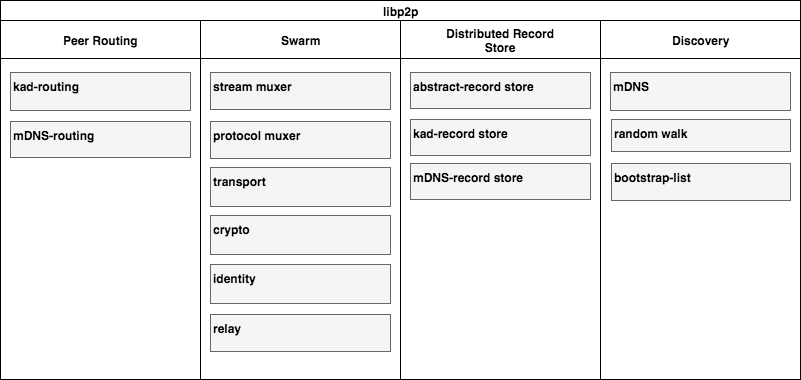
\includegraphics[width=0.45\textwidth]{libp2p-short.png}
\caption{Libp2p network stack}
\label{fig:libp2p-stack}
\end{figure}

The interfaces can be described as follows:
\begin{itemize}
\item \textbf{Peer Routing:} this identifies the peers to which a message should be routed.
The implementations include \textit{kad-routing}, a kademlia routing table where each peer holds a set of k-buckets; and mDNS-routing, which identifies local area network peers.
\item \textbf{Swarm:} this handles everything related to the opening of a stream.
A \textit{stream muxer}: this multiplexes connections per peer and streams per connection.
The \textit{protocol muxer}: enables the multiplexing of transport protocols on application levels.
This allows several protocols to be muxed in the same socket, in which case only one NAT traversal is required, if any.
Furthermore, \textit{Relay} provides an end-to-end encrypted connection where a node asks another node to connect on its behalf, enabling it to overcome NAT traversal.
\item \textbf{Distributed Record Store:} The aim is to store and distribute records; this activity is performed in a similar way to DNS as it is used for signaling links, and announcing peers and content.
The record store was further modularized under the name, InterPlanetary Record Store (IPRS)\cite{iprs}.
The interface provides record stores for abstract records, kademila routing records as well as mDNS routing records. 
Such a record keeping system allows content to be verified by any record store user.
\item \textbf{Discovery:} libp2p provides several ways for peers to find and identify each other in the network.
LAN discovery is implemented with \textit{mDNS}, \textit{Random Walk} using a DHT (distributed hash table) discovery, which executes random queries, which in turn enable the discovery of peers outside the LAN. 
Finally, a \textit{Bootstrap-list} enables peers to store highly stable (and possibly trusted) peers locally.

\end{itemize}

\subsection{Filecoin integration}
As at the time of writing, it is not known how Filecoin plans to adapt IPFS as its underlying data store.
Section \ref{subsec:ipfs-dfs} above introduced the components of IPFS briefly and provided a foundation for Filecoin to take advantage of the IFPS ecosystem.
We consider that the most obvious component to hook in is Bitswap (see Section \ref{subsec:ipfs-dfs}).
Bitswap manages requests from peers in the network and therefore is considered as the "data trading module" of IPFS \cite{bitswap}.
Essentially, Bitswap acquires blocks requested by the client and initiates a send to the peers who demand these blocks.
We believe that, in the case of Filecoin, the native measure of trust of Bitswap, as provided by the debt ratio factor, has to change.
Instead of relying on the number of bytes sent and received, Filecoin provides a measure of trust by relying on FIL token exchange and the guarantees provided by proof-of-spacetime (see Section \ref{subsec:pos}).
Therefore, in order to distribute the blocks among peers, Bitswap would react to \texttt{DEAL} orders (see Section \ref{subsec:ledger}).
Depending on whether the order emerged from the storage or retrieval market, blocks would be sent to the node corresponding to either the ask or the bid side.
As a result, Bitswap serves as the API used by the decentralized markets (see Section \ref{subsec:markets}) and handles data exchange according to Filecoin's incentive.

\section{Is the design economically feasible?}
\label{sec:eco-feasibility}

While analyzing the Filecoin ICO, people have also tried to measure the risk that comes with the investment.
Since there has not yet been any implementation, the investor has to rely on what is written in the Whitepaper and consider hypothetically the pros and cons of the project and the merits of its team members.
Therefore, the author of \cite{ico-analysis} has introduced a simple measure by adding (or subtracting) on a scale of 1 to 5 for every hypothetical pro (or con).
Table \ref{tbl:eco-risk} summarizes this work and extends it with the knowledge accumulated while writing this paper.
\begin{table}[H]
\centering
\caption{Estimation of economic feasibility}
\label{tbl:eco-risk}
\begin{tabular}{|l|l|}
\hline
\textbf{Aspect}                                                                                                                           & \textbf{Rating} \\ \hline
Image left after ICO                                                                                                                      & -2             \\ \hline
\begin{tabular}[c]{@{}l@{}}Overestimating the team's abilities \\ and/or underestimating the cost\end{tabular}                                 & -2             \\ \hline
\begin{tabular}[c]{@{}l@{}}Possible hurdles for the use of Filecoin \\ once ready\end{tabular}                                          & -3             \\ \hline
\begin{tabular}[c]{@{}l@{}}Ability to lure miners and customers \\ away from Storj and Siacoin due to\\ technical excellence\end{tabular} & +4             \\ \hline
\begin{tabular}[c]{@{}l@{}}Positioning for marketing opportunities \\ and business partnerships\end{tabular}                              & +3             \\ \hline
\begin{tabular}[c]{@{}l@{}}Response of the development team to user \\ demands\end{tabular}                                                  & +1             \\ \hline
\begin{tabular}[c]{@{}l@{}}Huge pool of free resources \\ made available by potential miners\end{tabular}                        & +2             \\ \hline
\end{tabular}
\end{table}
Our estimation shows that the biggest advantage of the project is its technical excellence in conjunction with its sophisticated marketing and its connectivity with other projects.
On the negative side, we see two major weaknesses:
first of all, the ICO left many investors and upcoming users with mixed feelings about the project.
We support the argument that the complexity of the implementation is likely to have been underestimated, and this has given rise to uncertainty; equally uncertain is the likelihood of users using the project at all.

\subsection{Is it a Ponzi scheme?}
Given that Filecoin raised a substantial amount of money with the ICO instrument, it is legitimate to raise the question of whether Filecoin itself is a Ponzi scheme.

By definition, a "Ponzi scheme" is a fraudulent investment operation that pays returns to its investors either from the investors' own money or from money paid by subsequent investors, rather than from any actual profit earned by the company. \cite{ponzi}

Indeed, in view of the information in Section \ref{sec:ico-analysis}, there are multiple factors which support this argument:
\begin{itemize}
\item Full control over investments by Protocol Labs (\ref{subsec:saft})
\item Exponentially higher return for early investors (\ref{subsec:token-sale})
\item Reward for vesting (\ref{sec:ico-analysis})
\item Lack of implementation
\end{itemize}

On the other hand, there are numerous logical reasons why an investor would \textit{trust} the people behind the Filecoin project:
The substantial technical capabilities of Protocol Labs have already been proven in the building of IPFS and libp2p; this could lead one to believe that their ability to overcome the upcoming hurdles in the building of Filecoin will be handled equally competently.
Furthermore, the investments raised are controlled by an intermediary (see \ref{sec:ico-analysis}), which holds connections to the SEC. 

The authors of this paper conclude that the proven technical capabilities of Protocol Labs should naturally be reason enough to believe that Filecoin is a legitimate project.
However, the terms and the way the ICO has proceeded are far from ideal.
Essentially, Protocol Labs allowed themselves to remain as the single entity that holds full control over the assets raised, without giving investors the possibility of intervening effectively.
Therefore, if goodwill fades, the entire project could turn into a Ponzi scheme.
\textit{Note: this is a hypothetical scenario and we are not implying that this scenario will occur. We are merely discussing possibilities.}

\subsection{A hypothetical comparison}

In view of the above, we would like to challenge the reader with speculation drawn from weakly supported statements and some hypothetical numbers.
The speculation is meant to be taken with a pinch of salt, however, it may also serve as an alert to the excessively bullish investor.

In a recent interview \cite{podcast}, Juan Benet compares Filecoin with Airbnb \cite{airbnb}, a website where people can rent out their homes (instead of disk storage).
Therefore, the following calculation compares the valuation of both companies against each other according to their resources.
Apartment space for Airbnb and disk space for Filecoin:
Airbnb is valued today (September 2017) at approximately \$31 billion while holding around 3 million listings in total \cite{airbnb-valuation}.
The average apartment in the United States was 934 square feet in 2016 \cite{housing-cnbc}.
In a hypothetical scenario, Airbnb is therefore valued at \$$11.06$ per square feet. 
If one compares this number to the median price per square foot in the United States, which is \$123 \cite{home-prices}, the Airbnb ecosystem diminishes the median price by a factor of $11.12$.
The average price for hard drives in 2017 is \$0.03 per gigabyte \cite{hard-drive}.
Dividing by the same factor that Airbnb applies for square feet to the storage price, the average gigabyte in the Filecoin system yields \$0.0027.
This means that the \$$257'000'000$ launched at the Filecoin ICO would require $95'185'185'185$ gigabytes ($95'185$ petabytes) of storage to be offered by storage miners.
Considering that Dropbox \cite{dropbox} currently holds around $500$ petabytes of user data \cite{dropbox-userdata}, one could argue that Filecoin is overvalued.

\section{Conclusion}
\label{sec:conclusion}

Projects such as Sia and StorJ have attracted attention by allowing people to provide and rent storage without any central party involved.
Filecoin's ICO began on August 10, 2017 and raised \$257 million, driven by investors who are also sympathetic to the idea of a decentralized storage market.

This paper now analyzes Filecoin's ICO and highlights some notable and disturbing facts.
For example, early investors, including Protocol Labs as the founder team, had to pay up to 8.57 times less than later investors.
Next, the Simple Agreement for Future Token (SAFT), signed by every investor, contains terms which strongly favor Protocol Labs.
It states that the invested money, none of which remains in the control of the investors, is refunded in cases which seem to be unlikely to occur. 
In addition, many of the terms have been defined in such a way as to minimize the sums which investors might expect to be returned.

Filecoin's technical capabilities, as described in the Whitepaper, have been studied in great detail.
We considered the details of the InterPlanetary File System (IPFS) project, a peer-to-peer hypermedia protocol which is used as the storage adapter for Filecoinm, with Filecoin serving as the incentivized layer.
It appears that IPFS can seamlessly serve as a storage adapter for Filecoin by introducing a new strategy for Bitswap whereas the orders define which peers shall serve data.
Further, we have raised the question of whether Filecoin is an economically feasible project firstly by extending the work of a hypothetical risk analysis, then considering the possibility of a Ponzi scheme, and finally with a simplified, hypothetical comparison with Airbnb.

Filecoin's economic feasibility is hard to predict and, given a simple summary of risk related points, the biggest hurdles are probably going to be acceptance from the users.
In addition, Filecoin shows certain characteristics of a Ponzi scheme but the trust built by the team members in the past leads us to believe that it is not one.
Filecoin's Whitepaper introduces novel concepts and predecessor projects by the team members which prove their technical capabilities.
Hence, it appears that Filecoin is poised to be an outstanding project although it remains to be seen if it will be adopted by the average cloud storage user.

% Can use something like this to put references on a page
% by themselves when using endfloat and the captionsoff option.
\ifCLASSOPTIONcaptionsoff
  \newpage
\fi

% trigger a \newpage just before the given reference
% number - used to balance the columns on the last page
% adjust value as needed - may need to be readjusted if
% the document is modified later
%\IEEEtriggeratref{8}
% The "triggered" command can be changed if desired:
%\IEEEtriggercmd{\enlargethispage{-5in}}

% references section

% can use a bibliography generated by BibTeX as a .bbl file
% BibTeX documentation can be easily obtained at:
% http://www.ctan.org/tex-archive/biblio/bibtex/contrib/doc/
% The IEEEtran BibTeX style support page is at:
% http://www.michaelshell.org/tex/ieeetran/bibtex/
%\bibliographystyle{IEEEtran}
% argument is your BibTeX string definitions and bibliography database(s)
%\bibliography{IEEEabrv,../bib/paper}
%
% <OR> manually copy in the resultant .bbl file
% set second argument of \begin to the number of references
% (used to reserve space for the reference number labels box)
\bibliographystyle{IEEEtran}

\bibliography{bibliography}

% that's all folks
\end{document}


